\chapter[ಅಧ್ಯಾಯ 10]{}\label{chap10}


\begin{center}
\rule{5cm}{1pt}\\[5pt]
{\Large\bfseries ಸಮಸ್ಯೆಗಳು}\\[3pt]
\rule{5cm}{1pt}
\end{center}

\begin{enumerate}
\renewcommand{\labelenumi}{\bf\theenumi.}
\itemsep=5pt

\item 1 ರಿಂದ 9 ವರೆಗಿನ ಅಂಕಿಗಳನ್ನು ಬೆಸ, ಸಮ - ಎರಡು ಗುಂಪುಗಳನ್ನಾಗಿ ವಿಭಾಗಿಸಿ. ಗುಂಪುಗಳ ಅಂಕಿಗಳನ್ನು ಮರುಜೋಡಿಸಿ, ಎರಡು ಗುಂಪುಗಳೂ ಪರಸ್ಪರ ಸಮ\-ವಾಗುವಂತೆ ಮಾಡಿ. ಯಾವುದೇ ಗಣಿತ ಪ್ರಕ್ರಿಯೆ ಬಳಸಬಹುದು. 

\item 0 ಯಿಂದ 9 ವರೆಗಿನ ಅಂಕಿಗಳನ್ನು ಯಾವುದೇ ರೀತಿಯಲ್ಲಿ ಜೋಡಿಸಿ 2 ಗುಂಪು ಮಾಡಿ ಗುಂಪುಗಳ ಮೊತ್ತ :- (ಭಿನ್ನರಾಶಿ ಬಳಸಬಹುದು)
\begin{itemize}
\item[(a)] 1 ಬರಬೇಕು 
\item[(b)] 100 ಬರಬೇಕು 
\end{itemize}

\item ನಾಲ್ಕು 7 ಬಳಸಿ 100 ಬರಿಸಿ. (ದಶಮಾಂಶ ಬಳಸಬಹುದು)

\item 1 ರಿಂದ 9 ವರೆಗಿನ ಅಂಕಿಗಳನ್ನು ಒಮ್ಮೆ ಮಾತ್ರ 99999 ಬರಿಸಿ. 

\item 5 ಬೆಸ ಸಂಖ್ಯೆ ಬಳಸಿ 20 ಬರಿಸಿ. ಅದೇ ಸಂಖ್ಯೆ ಮತ್ತೆ ಬಳಸಬಹುದು. 

\item ಮೂರಂಕಿಯ ಸಂಖ್ಯೆ ಪೂರ್ಣವರ್ಗ. ಅದರ ಅಂಕಿಗಳನ್ನು ಸ್ಥಾನ ಪಲ್ಲಟ ಮಾಡಿದರೆ ಬರುವ ಸಂಖ್ಯೆಯೂ ಪೂರ್ಣವರ್ಗ ಸಂಖ್ಯೆ ಯಾವುದು? 

\item ಒಂದು ಗೆರೆ ಸ್ಥಾನ ಪಲ್ಲಟ ಮಾಡಿ ಸಮೀಕರಣ ಸರಿದೂಗಿಸಿ $\neq$ ಬರುವಂತಿಲ್ಲ. 
\begin{itemize}
\item[(a)] VII $-$ IV = XII
\item[(b)] LV = X $-$ VL
\item[(c)] XI $+$ I = X
\end{itemize}


\item 5 ಬೆಂಕಿಕಡ್ಡಿ ಬಾಹುವಿನ ಒಂದು ಚೌಕವಿದೆ. ಮಧ್ಯದಲ್ಲಿ 1 ಬೆಂಕಿಕಡ್ಡಿ  ಚೌಕವಿದೆ. 
\begin{itemize}
\item[(a)] 18 ಬೆಂಕಿಕಡ್ಡಿ ಸೇರಿಸಿ 6 $`L'$ ಆಕೃತಿ (ಸಮಾನ ಅಳತೆ) ರಚಿಸಿ. 
\item[(b)] 20 ಬೆಂಕಿಕಡ್ಡಿ ಸೇರಿಸಿ 8$`L'$ ಆಕೃತಿ (ಸಮಾನ ಅಳತೆ) ರಚಿಸಿ. 
\end{itemize}

\begin{figure}[H]
\centering
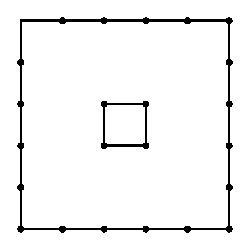
\includegraphics{images/chap10/q8.eps}
\end{figure}

\item 4 ಬೆಂಕಿಕಡ್ಡಿ ಬಾಹುವಿನ ಚೌಕವಿದೆ. 11 ಕಡ್ಡಿ ಸೇರಿಸಿ 4 ಭಾಗ ಮಾಡಬೇಕು. 

ಪ್ರತಿಭಾಗವೂ ಲಗತ್ತಾಗಿರಬೇಕು 1 ಭಾಗ ಚೌಕ, 2 $`L'$ ಆಕೃತಿ, 1 ಆಯತ, ಭಾಗಗಳ ವಿಸ್ತೀರ್ಣ 1ಕಡ್ಡಿ ಚದುರದ ನಾಲ್ಕರಷ್ಟು 

\begin{figure}[H]
\centering
\includegraphics{images/chap10/q9.eps}
\end{figure}

\item 3, 4, 5 ಕಡ್ಡಿ ಅಳತೆಯ ತ್ರಿಭುಜ ರಚಿಸಿ. 

(a) 3 ಕಡ್ಡಿ ಸ್ಥಳಾಂತರಿಸಿ, 1  ಕಡ್ಡಿ ಚದುರದ ನಾಲ್ಕರಷ್ಟಿರುವ ಆಕೃತಿ ರಚಿಸಿ. 

\item 12 ಕಡ್ಡಿಗಳಿಂದ ಈ ಆಕೃತಿ ರಚಿಸಿದೆ. 

\begin{minipage}[c]{5cm}
\begin{itemize}
\item[(a)] 2 ಕಡ್ಡಿ ಸ್ಥಾನ ಪಲ್ಲಟ ಮಾಡಿ 6 ಚೌಕ ಬರಿಸಿ. 
\item[(b)] 4 ಕಡ್ಡಿ ಸ್ಥಳಾಂತರಿಸಿ 3 ಚೌಕ ಬರಿಸಿ. 
\end{itemize}
\end{minipage}
\begin{minipage}[c]{4cm}
\begin{figure}[H]
\centering
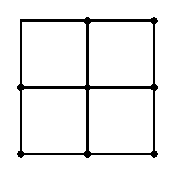
\includegraphics{images/chap10/q11.eps}
\end{figure}
\end{minipage}

\item ಈ ಗುಣಾಕಾರಗಳನ್ನು ಗಮನಿಸಿ. ಮುಂದಿನ 4 ಹಂತ ಬರೆಯಿರಿ. 
\begin{itemize}
\item[(a)]
\begin{tabular}[t]{rcl}
$0\times 9 + 1$ & = & $1$\\
$1\times 9 + 2$ & = & $11$\\
$12\times 9 + 3$ & = & $111$\\
$123\times 9 + 4$ & = & $1111$
\end{tabular}

\smallskip

\item[(b)]
\begin{tabular}[t]{ccc}
$9\times 9$ & = & $81$\\
$99\times 99$ & = & $9801$\\
$999\times 999$ & = & $998001$\\
$9999\times 9999$ & = & $99980001$
\end{tabular}

\smallskip

\item[(c)]
\begin{tabular}[t]{rcl}
$1 - 1$ & = & $9\times 0$\\
$11 - 2$ & = & $9\times 1$\\
$111 - 3$ & = & $9\times 12$\\
$1111 - 4$ & = & $9\times 123$
\end{tabular}
\end{itemize}

\item ಈ ಗುಣಾಕಾರ ಗಮನಿಸಿ 

\begin{tabular}[t]{ccl}
$1\times 23$ & = & $23$\\
$11\times 23$ & = & $253$\\
$111\times 23$ & = & $2553$\\
$1111\times 23$ & = & $25553$
\end{tabular}

\vskip 0.2cm

$1, 11, 111, 1111, \ldots$ ಈ ಸಂಖ್ಯೆಗಳನ್ನು ಯಾವುದೇ ಎರಡಂಕಿ ಸಂಖ್ಯೆಯಿಂದ (ಅಂಕಿಗಳ ಮೊತ್ತ 9ಕ್ಕಿಂತ ಹೆಚ್ಚಿರಬಾರದು) ಗುಣಿಸಿದರೆ, ಗುಣಲಬ್ಧದಲ್ಲಿ ಎರಡಂಕಿ ಗುಣಕದ ಅಂಕಿಗಳು ಮೊದಲು ಮತ್ತು ಕೊನೆಯಲ್ಲಿಯೂ, ಮಧ್ಯದಲ್ಲಿ, ಅವುಗಳ ಮೊತ್ತದ ಸಂಖ್ಯೆ, ಗುಣ್ಯದಲ್ಲಿನ 1ಗಳ ಸಂಖ್ಯೆಗಿಂತ 1ಸ ಕಡಿಮೆಯಾಗಿಯೂ ಬರುತ್ತದೆ. 

\vskip 0.1cm

ಇನ್ನೊಂದು ಉದಾಹರಣೆ ನೋಡಿ 

\begin{tabular}[t]{ccc}
$1\times 35$ & = & $35$\\
$11\times 35$ & = & $385$\\
$111\times 35$ & = & $3885$\\
$1111\times 35$ & = & $38885$
\end{tabular}

\vskip 0.2cm

ನೀವೂ ಪ್ರಯತ್ನಿಸಿ. ಇನ್ನೂ ಎರಡು ಗುಣಾಕಾರ ಬರೆಯಿರಿ. 6 ಹಂತ ಬರೆಯಿರಿ. ನೆನಪಿಡಿ ಎರಡಂಕಿ ಸಂಖ್ಯೆಯ ಅಂಕಿಗಳ ಮೊತ್ತ  9 ಮೀರಬಾರದು. 

\item ಈ ಗುಣಾಕಾರ ಗಮನಿಸಿ. ಮುಂದಿನ 3 ಹಂತ ಬರೆಯಿರಿ. 

{\fontsize{11pt}{13pt}\selectfont
\begin{tabular}[t]{ccl}
$9\times 0 + 8$ & = & $8$\\
$9\times 9 + 7$ & = & $88$\\
$9\times 98 + 6$ & = & $888$\\
$9\times 987 + 5$ & = & $8888$\\
\end{tabular}}\relax

\item ಈ ಗುಣಾಕಾರಗಳಲ್ಲಿ ಬರುವ ಮಾಲಾ ಸಂಖ್ಯೆ (Palindrome number) ಗಮನಿಸಿ. 

{\fontsize{11pt}{13pt}\selectfont
\begin{tabular}[t]{ccc}
$12\times 21$ & = & $252$\\
$112\times 211$ & = & $23632$\\
$1112\times 2111$ & = & $2347432$\\
$11112\times 21111$ & = & $234585432$
\end{tabular}}\relax

ಮುಂದಿನ ಹಂತದಲ್ಲಿ ಮಾಲಾ ಸಂಖ್ಯೆ ಬರುವುದೇ? ಪರೀಕ್ಷಿಸಿ. 

\item ಈ ಗುಣಾಕಾರಗಳನ್ನು ಗಮನಿಸಿ. 0ಯಿಂದ 9ರವರೆಗಿನ ಅಂಕಿಗಳು ಒಮ್ಮೆ ಮಾತ್ರ ಬಂದಿವೆ. 
{\fontsize{11pt}{13pt}\selectfont
\begin{tabbing}
$12\times 0483$ \= = \= $5796$\\
$04\times 1963$ \> =  \> $7852$
\end{tabbing}}\relax
ಇಂತಹ ಗುಣಾಕಾರ ರಚಿಸಲು ಯತ್ನಿಸಿ. 

\item 12 ನಾಣ್ಯಗಳನ್ನು 1 ಸಾಲಿನಲ್ಲಿ 5 ನಾಣ್ಯ ಇರುವ 3 ಸಾಲುಗಳಲ್ಲಿ ಜೋಡಿಸಿ. 

\item ಒಂದು ವೃತ್ತವನ್ನು 3 ಒಂದೇ ಉದ್ದದ ವಗ್ರ ರೇಖೆಗಳನ್ನೆಳೆದು 4 ಸಮ ಭಾಗ ಮಾಡಿ. 

\item ಒಂದು ವೃತ್ತಾಕಾರದ ಪಥ (track) ಇದೆ. ಅಗಲ 5 ಮೀ. ಒಂದು ಕುದುರೆ ಹೊರ ಅಂಚಿನಲ್ಲಿ ಓಡಿದಾಗ, ಒಳ ಅಂಚಿನಲ್ಲಿ ಅದೇ ವೇಗದಲ್ಲಿ ಓಡುವುದಕ್ಕಿಂತ $\Pi$ ಸೆಕೆಂಡ್ ಹೆಚ್ಚು ತೆಗೆದುಕೊಡರೆ, ಕುದುರೆಯ ವೇಗವೆಷ್ಟು? 

\item 9 ಸಸಿಗಳನ್ನು ಪ್ರತಿ ಸಾಲಿನಲ್ಲಿಯೂ 3 ಸಸಿ ಇರುವಂತೆ 10 ಸಾಲುಗಳಲ್ಲಿ ನೆಡಬೇಕು ಹೇಗೆ? 

\item 
\begin{tabular}[t]{ll}
&ಪಾರ್ಥ: ಕರ್ಣವಧಾಯ ಮಾರ್ಗಣಗಣಂ ಕೃದ್ಧೋರಣೇ ಸಂಧದೇ ।\\
&ತಸ್ಯಾರ್ಧೇನ ನಿನಾರ್ಯ ತಚ್ಛರಗಣಂ ಮೂಲೈ ಚತುರ್ಭಿರ್ಹಯಾನ್ ।।\\
&ಶಲ್ಯಂ ಷಡ್ಭಿರಧೇಷ ಭಿ ಸ್ತ್ರಿ ಭಿರತಿ ಚ್ಛತ್ರಂ ಧ್ವಜಂ ಕಾರ್ಯುಕಂ ।\\
&ಚಿ ಚ್ಛೇದಾಸ್ಯ ಶಿರಃ ಶರೇಣ ಕತಿತೇಯಾನರ್ಜುನಃ ಸಂದಧೇ ।।\\
&\hfill{(ಭಾಸ್ಕರಾಚಾರ್ಯರ `ಲೀಲಾವತೀ'ಯಿಂದ)}
\end{tabular}

\vfill\eject

ಪಾರ್ಥನು ಕೋಪಾವಿಷ್ಟನಾಗಿ ಕರ್ಣನ ವಧೆಗಾಗಿ ರಣರಂಗದಲ್ಲಿ ನಿರತನು. ಬತ್ತಳಿಕೆಯಲ್ಲಿನ ಬಾಣಗಳಲ್ಲಿ ಅರ್ಧ ಸಂಖ್ಯೆಯನ್ನು ಶತ್ರು ಶರ ನಿವಾರಣೆಗಾಗಿ ಪ್ರಯೋಗಿಸಿದನು. ವರ್ಗ ಮೂಲದ ನಾಲ್ಕರಷ್ಟರಿಂದ ಶತ್ರುವಿನ ಕುದುರೆಗಳನ್ನು ಕೊಂದನು. ಶಲ್ಯನಿಗೆ ಆರು ಬಾಣಗಳಾದುವು. ಮೂರರಿಂದ ಕರ್ಣನ ಧ್ವಜ, ಛತ್ರ, ಬಿಲ್ಲುಗಳು ಉರುಳಿದುವು. ಉಳಿದ ಒಂದು ಬಾಣವು ಕರ್ಣನ ಶಿರಚ್ಛೇದನ ಮಾಡಿತು. ಒಟ್ಟು ಎಷ್ಟು ಬಾಣಗಳಿದ್ದುವು. 

\item ದಾರ್ಧಂ ತಂಡುಲ ಮಾರ್ನ ತ್ರಯ ಮಹೋದ್ರಮ್ಮೇಣ ಮಾನಾಷ್ಟಕಂ ।

ಮುದ್ಗಾನಾಂಚ ಯದಿ ತ್ರಯೋದಶಮಿತಾ ಏತಾವಣಕ್ಕಾಕಿನೀ 

ಆದಾಯಾರ್ಪಯ ತಂಡುಲಾಂಶಿ ಯುಗಲಂ ಮುದ್ಗೈಕ ಭಾಗಾನ್ವಿತಂ 

ಕ್ಷಿಪಂ ಕ್ರಿಪ್ರಭುಜೋ ಪ್ರಜೇಮಹಿಯತಃ ಸಾರ್ಥೇಗ್ರತೋಯಾಸ್ಯತಿ ।।

\smallskip

\hfill{(ಭಾಸ್ಕರಾಚಾರ್ಯರ `ಲೀಲಾವತೀ'ಯಿಂದ)}

\smallskip

ಒಂದು ದ್ರಮ್ಮಕ್ಕೇ $3\frac{1}{2}$ ಮಾನಗಳಷ್ಟು ಅಕ್ಕಿ ಅಥವಾ 8ಮಾನಗಳಷ್ಟು ಉದ್ದು ಬರುತ್ತದೆ. ಎಲೈ ವರ್ತಕನೇ, ಈ 13 ಕಾಕನಿಗಳಿಗೆ 2 ಭಾಗ ಅಕ್ಕಿ, ಒಂದು ಭಾಗ ಉದ್ದು ಇರುವಂತೆ ಈ ಧಾನ್ಯಗಳನ್ನು ಬೇಗನೆ ಕೊಂಡು ನಮ್ಮ ಗುಂಪಿನವರು ಮುಮ್ದಕ್ಕೆ ಪ್ರಯಾಣ ಬೆಳಸುತ್ತಾರಾದ್ದರಿಂದ, ನಾವು ಅವಸರದಿಂದ ಊಟ ಮಾಡಿಕೊಂಡು ಹೊರಡಬೇಕಾಗಿದೆ. 

\{ನಾಣ್ಯಗಳ ಕೋಷ್ಟಕಃ 20 ವರಾಟಕ = 1 ಕಾಕಿನಿ, 4 ಕಾಕಿನಿ  = 1 ಪಣ, 16 ಪಣ = 1 ದ್ರಮ್ಮ, 16 ದ್ರಮ್ಮ  = 1 ನಿಷ್ಕ\}  

\item ಒಂದು ಬಕೆಟ್‌ನ ತಳ ಮತ್ತು ಮೇಲ್ಭಾಗದ ಭಾಗಗಳ ತ್ರಿಜ್ಯಗಳು ಕ್ರಮವಾಗಿ 7ಸೆ.ಮೀ ಮತ್ತು 28 ಸೆ.ಮೀ. ಇವೆ ಬಕೆಟ್‌ನ ಎತ್ತರ 45 ಸೆ.ಮೀ ಬಕೆಟ್‌ನ ಹಿಡಿಪು (capacity) ಮತ್ತು ಮೇಲ್ಮೈ ವಿಸ್ತೀರ್ಣ ಕಂಡು ಹಿಡಿಯಿರಿ. 

\item ಒಂದು ಆಯತಾಕಾರದ ಲೋಹದ ಹಾಳೆ 48 cm ಉದ್ದ 36 cm ಅಗಲವಿದೆ. ಅದರ ನಾಲ್ಕು ಮೂಲೆಗಳಲ್ಲೂ 8 cm ಚೌಕದಷ್ಟು ಹಾಳೆ ಕತ್ತರಿಸಿದೆ. ಉಳಿದ ಭಾಗದಿಂದ\break ಒಂದು ತೆರೆದ ಡಬ್ಬ ಮಾಡಿದೆ. ಡಬ್ಬದ ಹಿಡಿಪು (capcity) ಲೆಕ್ಕಿಸಿ. 

\item ಇಬ್ಬರು ಸೈಕಲ್ ಸೂರರ ನಡುವೆ $\frac{1}{2}$ km ಅಂತರವಿದೆ. ಒಬ್ಬ 6 KMPH ಒಬ್ಬನು 6 KMPH ಮತ್ತು ಇನ್ನೊಬ್ಬನು 4 KMPH ನಲ್ಲಿ ಎದುರು ಬದುರಾಗಿ ಬರುತ್ತಿದಾರೆ. ಒಂದು ನೊಣ 20 KMPH ವೇಗದಲ್ಲಿ ಅವರಿಬ್ಬರ ನಡುವೆ ಒಬ್ಬರಿಂದ ಇನ್ನೊಬ್ಬರಿಗೆ ಹಿಂದಕ್ಕೆ ಮುಂದಕ್ಕೆ ಹಾರಾಡುತ್ತಿದೆ. ಅವರಿಬ್ಬರೂ ಸಂಧಿಸಿದಾಗ, ನೊಣ ಎಷ್ಟು ದೂರ ಹಾರಿತ್ತು? 

\item ಇದೊಂದು ಅಪೂರ್ಣ ಮಾಯಾಚೌಕ. ಮಾಯಾಚೌಕದಲ್ಲಿ ಅಡ್ಡ ಸಾಲು, ಕಂಭ ಸಾಲು, ಕರ್ಣಗಳಲ್ಲಿನ ಸಂಖ್ಯೆಗಳ ಮೊತ್ತ ಸಮನಾಗಿರುತ್ತದೆ. ಈ ಅಪೂರ್ಣ ಚೌಕವನ್ನು ಪೂರ್ಣಗೊಳಿಸಿ. ಇದು ಏಕಕಾಲಿಕ ಸಮೀಕರಣಗಳ ಮೇಲಿನ ಲೆಕ್ಕ 
\begin{figure}[H]
\centering
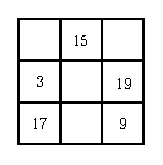
\includegraphics[scale=1.2]{images/chap10/q26.eps}
\end{figure}
 
\item 10 ಬಿಲ್ಲೆಗಳ ಜೋಡಣೆ ಹೀಗಿದೆ ಯಾವುದಾದರೂ 3 ಬಿಲ್ಲೆ ಸ್ಥಾನ ಪಲ್ಲಟಮಾಡಿ ಪಿರಮಿಡ್ ಶೃಂಗ ಮೇಲೆ ಬರಿಸಿ. 
\begin{figure}[H]
\centering
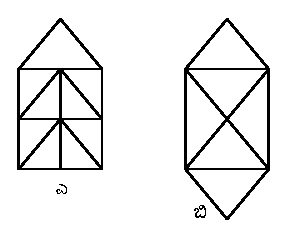
\includegraphics[scale=1.2]{images/chap10/q27.eps}
\end{figure}

\item ಈ ವರ್ಗ ಸಂಖ್ಯೆಗಳ ವಿಶಿಷ್ಟತೆ ಗಮನಿಸಿ. 

\begin{tabular}[t]{rcl}
$88^{2}$ & = & $7744$\\
$8989^{2}$ & = & $8080~21~21$\\
$406406^{2}$ & = & $165~165~836~836$\\
$593593^{2}$ & = & $382~382~649~649$\\
$998998^{2}$ & = & $997~997~004~004$
\end{tabular}

\item ಈ ಲೆಕ್ಕ ಗಮನಿಸಿ. ಮುಂದಿನ 3 ಹಂತ ಬರೆಯಿರಿ. 

\begin{tabular}[t]{ccl}
$57^{2} - 54^{2}$ & = & $333$\\
$557^{2} - 554$ & = & $3333$\\
$5557^{2} - 5554$ & = & $33333$
\end{tabular}

\item ನಾಲ್ಕಂಕಿಯ ಒಂದು ಸಂಖ್ಯೆ. ಅದು 1287 ರಿಂದ ನಿಶ್ಶೇಷವಾಗಿ ಭಾಗವಾಗುತ್ತದೆ. ಅಂಕಿಗಳು $- 8 - -$. ಉಳಿದ ಅಂಕಿಗಳನ್ನು ಪತ್ತೆಮಾಡಿ.  
\end{enumerate}


\begin{center}
\rule{5cm}{1pt}\\[3pt]
{\Large\bfseries ಉತ್ತರಗಳು}\\[-0.1cm]
\rule{5cm}{1pt}
\end{center}

\begin{enumerate}
\itemsep=5pt

\item ಎರಡು ಗುಂಪುಗಳು 1, 3, 5, 7, 9 ಮತ್ತು 2, 4, 6, 8

$79 + 5\dfrac{1}{3} = 84 + \dfrac{2}{6} = 84\dfrac{1}{3}$

\item 
\begin{itemize}
\item[(a)] $\dfrac{35}{70} + \dfrac{148}{296} = \dfrac{1}{2} + \dfrac{1}{2} = 1$

\medskip

\item[(b)] $98 \dfrac{27}{54} + 1\dfrac{3}{6} = 98\dfrac{1}{2} + 1\dfrac{1}{2} = 100$
\end{itemize}

\item $\dfrac{7}{7}\times \dfrac{7}{7} = 10\times 10 = 100$

\smallskip
\item $98765 + 1234 = 99999$

\item $13 + 3 + 3 + 1 = 20$

\item 

\begin{tabular}[t]{lll}
$196 = 14^{2}$ & $144 = 12^{2}$ & $256 = 16^{2}$\\
$961 = 31^{2}$ & $441 = 21^{2}$ & $625 = 25^{2}$\\
$169 = 13^{2}$, & $961 = 31^{2}$, & $196 = 14^{2}$
\end{tabular}

\item 
\begin{itemize}
\item[(a)] VII $+$ V = XII (IVಯ 1ನ್ನು $-$ ಮೇಲೆ ಇಟ್ಟಿದೆ.)
\item[(b)] LV $-$ X = VL (=ನ ಒಂದುಗೆರೆಯನ್ನು $-$ ಮೇಲೆ ಇಟ್ಟಿದೆ.)
\item[(c)] X $+$ I = XI (XIನ 1ಗೆರೆಯನ್ನು X ನ ಮುಂದೆ ಬರೆದಿದೆ.)
\end{itemize}

C ಇನ್ನೊಂದು ಉತ್ತರ IX $+$ I = X

\item 
~

\begin{minipage}[c]{4.5cm}
\begin{figure}[H]
\centering
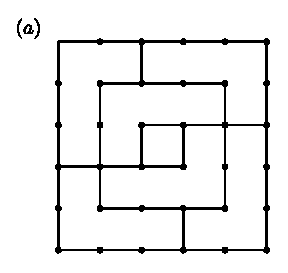
\includegraphics{images/chap10/ans8a.eps}
\end{figure}
\end{minipage}
\begin{minipage}[c]{4.5cm}
\begin{figure}[H]
\centering
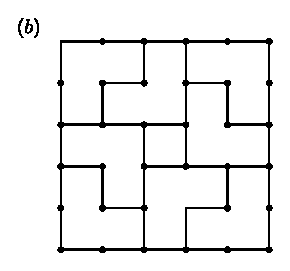
\includegraphics{images/chap10/ans8b.eps}
\end{figure}
\end{minipage}

\item 
~

\begin{minipage}[c]{4cm}
\begin{figure}[H]
\centering
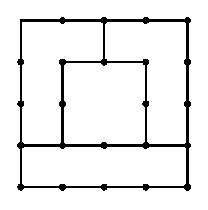
\includegraphics{images/chap10/ans9.eps}
\end{figure}
\end{minipage}
\begin{minipage}[c]{5cm}
ಚೌಕ $2\times 2$ ಒಂದು \\
$`L'$ ಆಕೃತಿ 2 (4 ಒಂದು ಕಡ್ಡಿ ಚೌಕ ಅಳತೆ)\\
ಆಯತ 1 ($1\times 4$ ಕಡ್ಡಿ ಅಳತೆ)
\end{minipage}


\item ಕೊಟ್ಟಿರುವುದು 

\begin{minipage}[c]{7cm}
\begin{figure}[H]
\centering
\hspace{4cm}\text{ರಚನೆ }

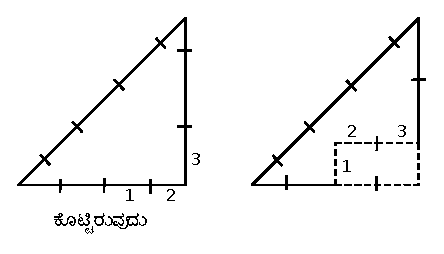
\includegraphics{images/chap10/ans10.eps}
\end{figure}
\end{minipage}
\begin{minipage}[c]{2cm}
3 ಕಡ್ಡಿ \\
ಸ್ಥಳಾಂತರಿಸಿದೆ. 
\end{minipage}

\begin{gather*}
\text{ತ್ರಿಭುಜದ ವಿಸ್ತೀರ್ಣ}~ \dfrac{4\times 3}{2} = 6 \text{ ಚ.ಕಡ್ಡಿಗಳು}\\
\text{ಕಡಿಮೆಯಾಗಿರುವುದು}~ 2\times 1 = 2 \text{ ಚ.ಕಡ್ಡಿಗಳು}\\
\text{ಉಳಿಕೆ}~ 6 - 2 = 4 \text{ ಚ.ಕಡ್ಡಿಗಳು}
\end{gather*}

\item 
~

\begin{minipage}[c]{5cm}
\begin{figure}[H]
\centering
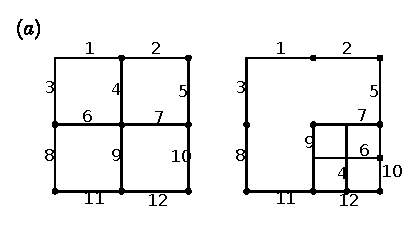
\includegraphics{images/chap10/ans11a.eps}
\end{figure}
\end{minipage}
\qquad\qquad
\begin{minipage}[c]{4cm}
4, 6 ಸ್ಥಳಾಂತರಿಸಿದೆ

\begin{tabular}{l}
$\frac{1}{2}$ ಕಡ್ಡಿ ಚೌಕಗಳು $4$\\
$1$ ಕಡ್ಡಿ ಚೌಕ  $1$\\
$2$ ಕಡ್ಡಿ ಚೌಕ  $1$\\
\end{tabular}
\end{minipage}


\begin{minipage}[c]{4cm}
\begin{figure}[H]
\centering
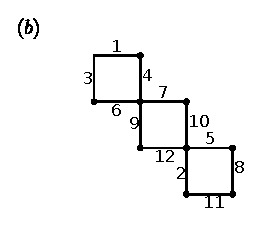
\includegraphics{images/chap10/ans11b.eps}
\end{figure}
\end{minipage}
\begin{minipage}[c]{5cm}
2, 5, 8, 11 ಕಡ್ಡಿಗಳನ್ನು \\
ಮರು ಜೋಡಿಸಿದೆ. \\
3 ಚೌಕಗಳು. 
\end{minipage}

\item 
\begin{itemize}
\item[(a)]
\begin{tabular}[t]{rcl}
$1234\times 9 + 5$ & = & $111~11$\\
$12345\times 9 + 6$ & = & $111~111$\\
$123456\times 9 + 7$ & = & $111~111~1$\\
$1234567\times 9 + 8$ & = & $111~111~11$
\end{tabular}

\vskip 0.3cm

\item[(b)]
\begin{tabular}[t]{rcl}
$99999\times 99999$ & = & $99998~00001$\\
$999~999\times 999~999$ & = & $999998~000001$\\
$999~999~9\times 999~999~9$ & = & $9999998~000~0001$\\
$9999~9999\times 9999~9999$ & = & $999~999~98~000~00001$
\end{tabular}

\vskip 0.3cm

\item[(c)]
\begin{tabular}[t]{rcl}
$111~11 - 5$ & = & $9\times 1234$\\
$111~111 - 6$ & = & $9\times 12345$\\
$111~111~1 - 7$ & = & $9\times 123456$\\
$1111~1111 - 8$ & = & $9\times 1234567$
\end{tabular}	
\end{itemize}

\vskip 0.3cm

\item 

{\fontsize{10pt}{12pt}\selectfont
\begin{tabular}[t]{rcl}
$1\times 72$ & = & $72$\\
$11\times 72$ & = & $792$\\
$111\times 72$ & = & $7992$\\
$1111\times 72$ & = & $79992$\\
$11111\times 72$ & = & $799992$\\
$111111\times 72$ & = & $7999992$
\end{tabular}}\relax

\smallskip

{\fontsize{10pt}{12pt}\selectfont
\begin{tabular}[t]{rcl}
$1\times 61$ & = & $61$\\
$11\times 61$ & = & $671$\\
$111\times 61$ & = & $6771$\\
$1111\times 61$ & = & $67771$\\
$11111\times 61$ & = & $67771$\\
$111111\times 61$ & = & $677771$
\end{tabular}}\relax

\item 
\begin{tabular}[t]{lll}
$9\times 9876 + 4$ & = & $888~88$\\
$9\times 98765 + 3$ & = & $888~888$\\
$9\times 987654 + 2$ & = & $888~8888$\\
$9\times 9876543 + 1$ & = & $8888~8888$\\
\end{tabular}

\item ಉತ್ತರದ ಅಗತ್ಯವಿಲ್ಲ 

\item 
\begin{tabular}[t]{lll}
$18\times 0297$ & = & $5346$\\
$39\times 0186$ & = & $7254$\\
$48\times 0159$ & = & $7632$
\end{tabular}

\item 
~

\begin{figure}[H]
\centering
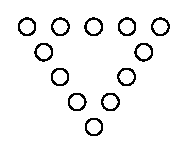
\includegraphics{images/chap10/ans17.eps}
\end{figure}

\item 
~

\begin{figure}[H]
\centering
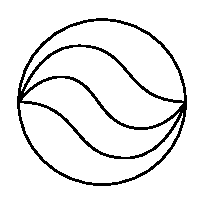
\includegraphics{images/chap10/ans18.eps}
\end{figure}

\item 
~

\begin{minipage}[c]{5cm}
ಒಳ ವೃತ್ತದ ತ್ರಿಜ್ಯ $`r'$ ಇರಲಿ 

ಪರಿಧಿ $2\pi r$ ಮೀ. 

ಹೊರ ವೃತ್ತದ ತ್ರಿಜ್ಯ $(r + 5)$ ಮೀ

ಪರಿಧಿ $2\Pi (r + 5)$ ಮೀ

ಕುದುರೆಯ ವೇಗ $`t'$ ಮೀ/ಸೆ. ಇರಲಿ.

ಒಳಗಡೆ ಓಡುವ ಕಾಲ $\dfrac{2\Pi r}{t}$ ಸೆ ~;

ಹೊರಗಡೆ ಓಡುವ ಕಾಲ $\dfrac{2\Pi (r + 5)}{t}$ ಸೆ.   
\end{minipage}
\qquad
\begin{minipage}[c]{4cm}
\begin{figure}[H]
\centering
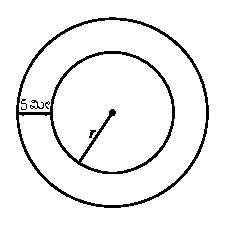
\includegraphics[scale=1.1]{images/chap10/ans19.eps}
\end{figure}
\end{minipage}

\begin{align*}
\dfrac{2\Pi (r + 5)}{t} - \dfrac{2\Pi r}{t} & = \Pi\\
\dfrac{\cancel{2\Pi r} + 10\Pi - \cancel{2\Pi r}}{t} & = \Pi\\
\dfrac{10\Pi}{t} & = \Pi\\
10\Pi & = t\Pi \quad or\quad t = 10 \text{ ಮೀ/ಸೆ.}
\end{align*}

\item 
~

\begin{minipage}[c]{4cm}
\begin{figure}[H]
\centering
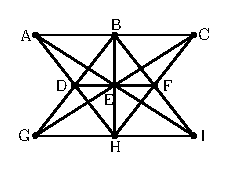
\includegraphics[scale=1.2]{images/chap10/ans20.eps}
\end{figure}
\end{minipage}
\begin{minipage}[c]{5cm}
\begin{align*}
& \left.
\begin{aligned}
& A, B, C, D, E\\
& F, G, H, I 
\end{aligned}
\right\}
\quad\text{$9$ ಸಸಿಗಳು}\\
& AC, AH, AI \\
& BE, BH, BJ \\
& AH, AI \\
& CG, CH
\end{align*}
\end{minipage}

\item ಪಾರ್ಥನಲ್ಲಿದ್ದ ಬಾಣಗಳು $x$ ಇರಲಿ 
\begin{gather*}
\dfrac{1}{2}x + 4\sqrt{x} + 6 + 3 + 1 = x\\
8\sqrt{x} = x - 20\\
\end{gather*}

ವರ್ಗವಣೆಯಿಂದ\quad $64x = x^{2} - 40x + 400$
\begin{gather*}
x^{2} - 104x + 400 = 0\\
(x - 100) (x - 4) = 0\\
x = 100 \quad\text{ ಅಥವಾ}~ 4
\end{gather*}
4 ಶಲ್ಯನಿಗೆ ಸಾಲುವುದಿಲ್ಲ $~\therefore\quad$ ಉತ್ತರ 100 ಬಾಣಗಳು 

\item 1 ದ್ರಮ್ಮ = 16 ಪಣ =  64 ಕಾಕಿನಿ 

\begin{tabular}[t]{ll}
$64$ ಕಾಕನಿಗೆ & $3\dfrac{1}{2}$ ಮಾನ ಅಕ್ಕಿ \\
$64$ ಕಾಕನಿಗೆ & $8$ ಮಾನ ಉದ್ದು \\[0.3cm]
$\therefore 1$ ಮಾನ ಅಕ್ಕಿಗೆ & $\dfrac{64\times 2}{7}$ ಕಾಕಿನಿ\\
$1$ ಮಾನ ಉದ್ದಿಗೆ ಕಾಕಿನಿ  & $8$ ಕಾಕಿನಿ 
\end{tabular}

\vskip 0.3cm

$2$ ಮಾನ ಅಕ್ಕಿಗೆ $\dfrac{256}{7}$ ಕಾಕಿನಿ $d$

($2$ ಮಾನ ಅಕ್ಕಿ $+ 1$ ಮಾನ ಉದ್ದು) ಬೆಲೆ = $\dfrac{256}{7} + \dfrac{8}{1} = \dfrac{312}{7}$ ಕಾಕನಿ 

$\dfrac{312}{7}$ ಕಾಕಿನಿಗೆ ($2$ ಮಾನ ಅಕ್ಕಿ $+ 1$ ಮಾನ ಉದ್ದು ) ಸಿಗುತ್ತದೆ. 

$13$ ಕಾಕಿನಿಗೆ  $\dfrac{7\times 13}{312} = \dfrac{7}{24}$ ಭಾಗಲಬ್ಧ 

$\dfrac{7}{24}$ ಭಾಗ ಉದ್ದು, $\dfrac{7}{12}$ ಭಾಗ ಅಕ್ಕಿ 

\smallskip

\item 
~

\begin{minipage}[c]{4cm}
\begin{equation*}
\left.
\begin{aligned}
\text{ಬಕೆಟ್‌ನ ಮೇಲ್ಭಾಗದ ತ್ರಿಜ್ಯ}  ~R \\
\text{ಕೆಳಭಾಗದ ತ್ರಿಜ್ಯ} ~r   \\
\text{ಎತ್ತರ} ~h  
\end{aligned}
\right\}
\text{ಇದ್ದರೆ}
\end{equation*}
\end{minipage}
\qquad
\begin{minipage}[c]{5cm}
\begin{figure}[H]
\centering
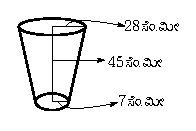
\includegraphics{images/chap10/ans23.eps}
\end{figure}
\end{minipage}

\smallskip

ಹಿಡಿಪು (ಗಾತ್ರ) $V = \dfrac{\phi}{3} (R^{2} + r^{2}  Rr)$

ಮೇಲ್ಮೇ ವಿಸ್ತೀರ್ಣ $= \Pi (L(R + r) + r^{2})$

${l = \dfrac{{\text{ ಸೂತ್ರಗಳು }}}{\sqrt{h^{2} + (R - r)^{2}}}}$
\begin{align*}
\text{ ಗಾತ್ರ} & = \dfrac{22}{7} \times \dfrac{45}{3} (28^{2} + y^{2} + 28 + 7)\\
& = \dfrac{22\times 15}{7} (784 + 49 + 196)\\
& = \dfrac{22}{7} \times 15\times 1029 = 48510 ~~\text{ಸೆಂ.ಮೀ.}^{3}\\
L & = \sqrt{45^{2} + (28^{2} - 7^{2})} = \sqrt{45^{2} + 21^{2}} \\
&= \sqrt{2466} = 49.66\\
& \therefore\quad \text{ಮೇಲ್ಮ್ಯೆ  ವಿಸ್ತೀರ್ಣ:}\\
& \dfrac{22}{7} (49.66\times 35 + 49) \\
& = 5616.6 \text{ ಸೆಂ.ಮೀ}^{2} 
\end{align*}

\item
~

\begin{minipage}[c]{6cm}
ತೆರೆದ ಡಬ್ಬದ ಉದ್ದ $(48 - 8 - 8) = 26$ cm\\
ಅಗಲ $(36 - 8 - 8) = 20$ cm\\
ಎತ್ತರ $8$ cm
\end{minipage}
\begin{minipage}[c]{3cm}
\begin{figure}[H]
\centering
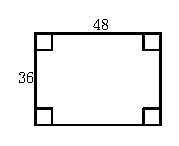
\includegraphics{images/chap10/ans24.eps}
\end{figure} 
\end{minipage}

\vskip 0.3cm

$\therefore~$ ಹಿಡುಪು (ಗಾತ್ರ) = L $\times$  B$\times$ H $= 26\times 20\times 8 = 4160$ cm$^{3}$

\item  ಇಬ್ಬರು ಸವಾರರ ಒಟ್ಟು ವೇಗ ($6 + 4$) KMPH ಅವರ ನಡುವಿನೆ ಅಂತರ $\dfrac{1}{2}$ KM

$10$ ಕಿ.ಮೀ ಗೆ  $1$ ಗಂ. $\quad\therefore\quad \dfrac{1}{2}$ ಕಿ.ಮೀ ಗೆ $\dfrac{1}{20}$ ಗಂ 

\vskip 0.2cm

ನೊಣ $20$ KMPH ಹಾರಾಡುತ್ತದೆ. 

$\dfrac{1}{20}$ ಗಂಟೆಯಲ್ಲಿ $1$ ಕಿ.ಮೀ ಹಾರಾಡುತ್ತದೆ. 

\vskip 0.5cm

\item 
~

\begin{minipage}[c]{4cm}
\begin{figure}[H]
\centering
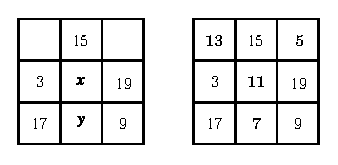
\includegraphics[scale=1.3]{images/chap10/ans26.eps}
\end{figure} 
\end{minipage}
\begin{minipage}[c]{5cm}
ಮಧ್ಯದ ಕಂಬ ಸಾಲಿನ ಸಂಖ್ಯೆಗಳು \\ 
$x$, $y$ ಇರಲಿ 
\end{minipage}

\begin{minipage}[c]{5cm}
\begin{align*}
\text{ಈಗ}\quad 3 + x + 19 & = 17 + y + 9 \\
& = 15 + x + y \text{ ನಿದಿಸುತ} \\
x + 22 & = x + y + 15\\
\therefore~ y & = 22 - 15 = 7\\
\therefore~ x & = 11
\end{align*}

ಉತ್ತರಗಳನ್ನು ತುಂಬಿಸಿದೆ. 
\end{minipage}
\begin{minipage}[c]{4cm}
\begin{figure}[H]
\centering
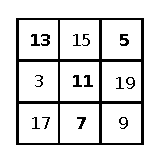
\includegraphics[scale=1.1]{images/chap10/ans26a.eps}
\end{figure} 
\end{minipage}


\item ಕೊಟ್ಟಿರುವುದು 

\begin{minipage}[c]{5cm}
\begin{figure}[H]
\centering
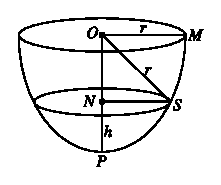
\includegraphics{images/chap10/ans27.eps}
\end{figure}
\end{minipage}
\begin{minipage}[c]{4cm}
1, 4, 10\\
ಸ್ಥಾನ ಪಲ್ಲಟ ಮಾಡಿದೆ 
\end{minipage}

\item ಉತ್ತರದ ಅಗತ್ಯವಿಲ್ಲ 

\item 
\begin{tabular}[t]{ccl}
$55557^{2} - 55554^{2}$ & = & $333~33$\\
$555557^{2} - 555554^{2}$ & = & $333~333$\\
$555~5557^{2} - 555~5554^{2}$ & = & $333~3333$
\end{tabular}

\item 1287 ರ ಅಪವರ್ತನಗಳು 9, 11, 13. ಇವುಗಳಲ್ಲಿ ಪ್ರತಿಯೊಂದರಿಂದಲೂ ಭಾಗವಾಗಬೇಕು. ಸಂಖ್ಯೆಯ ಬಿಡಿಸ್ಥಾನದ ಅಂಕಿ 1 ಇರಬೇಕು 

$\therefore\quad$ ಸಂಖ್ಯೆ  $ - 8 - 1$

11 ರಿಂದ ಭಾಗವಾಗಬೇಕಾದರೆ $8 + 1$ = ಉಳಿದೆರಡು ಅಂಕಿಗಳ ಮೊತ್ತ 

$\therefore\quad$ ಉಳಿದ ಸ್ಥಾನಗಳ ಅಂಕಿಗಳು $1, 8 ~;~ 2, 7 ~;~ 3, 6 ~;~ 4, 5$ ಇರಬೇಕು. ಇವುಗಳನ್ನು ತುಂಬಿಸಿ ನೋಡಿ. 3, 6 ಸರಿಯಾಗುತ್ತದೆ. $\therefore~$ ಸಂಖ್ಯೆ 3861

$(1287\times 3 = 3861)$
\end{enumerate}
